\documentclass[noexaminfo,oneside,binding=0.6cm]{sapthesis}
\usepackage[T1]{fontenc}
\usepackage[utf8]{inputenc}
\usepackage[italian]{babel}
\usepackage{array}
\usepackage{float}
\usepackage{booktabs}
\usepackage{tabularx}
\usepackage{listings}
\usepackage{xcolor}
\definecolor{lightgray}{rgb}{0.95,0.95,0.95}
\lstset{
  language=C,                         
  basicstyle=\ttfamily\small,        % font size and style
  backgroundcolor=\color{lightgray}, % background color
  frame=single,                      % adds a box around code
  rulecolor=\color{gray},           % color of frame
  numbers=left,                     % show line numbers
  numberstyle=\tiny\color{gray},    % style of line numbers
  numbersep=10pt,                   % space between code and line numbers
  keywordstyle=\color{blue},        % style for keywords
  commentstyle=\color{green!50!black}, % style for comments
  stringstyle=\color{red},          % style for strings
  tabsize=4,                         % tab width
  showstringspaces=false,           % don't show spaces in strings
  breaklines=true,                  % automatic line breaking
  breakatwhitespace=true,           % only break at white space
  captionpos=b                      % caption position (t or b)
}

\usepackage{lipsum}
\usepackage{url}
\usepackage{graphicx}
\usepackage{placeins}
\usepackage{wrapfig}
\usepackage{hyperref}
\usepackage{multicol,caption}
\usepackage[bottom]{footmisc}

\title{Implementazione di un allocatore di memoria bare metal in C}
% \alttitle{A study on Memory Allocators}
\subtitle{Come ho imparato a non preoccuparmi e ad amare l'allocatore}
\author{Antonio Turco}
\IDnumber{1986183} 
\date{\today}
\course{Corso di Laurea Triennale in Ingegneria Informatica e Automatica}  
\courseorganizer{Facoltà di Ingegneria dell'Informazione, Informatica e Statistica}
\AcademicYear{2024/2025}
\advisor{Prof. Giorgio Grisetti}
\copyyear{2024/2025}
\versiondate{\today}
\authoremail{turco.1986183@studenti.uniroma1.it}

\begin{document}

\frontmatter  
\maketitle
\dedication{Dedicato a...}

\begin{abstract}
  ABSTRACT HERE
\end{abstract}


\mainmatter 
\tableofcontents

\chapter{Introduzione}
\begin{itemize}
  \item Cos’è la memoria dinamica? In cosa consiste la sua gestione?
  \item Qual è il ruolo dell’allocatore di memoria?
  \item Quali sono le metriche che distinguono un buon allocatore da un allocatore inefficiente?
  \item Perché è importante che l’allocatore di memoria sia efficiente? In quali contesti è essenziale?
  \item Quali sono le diverse tipologie di allocatori di memoria?
\end{itemize}

\chapter{Letteratura esistente sull'argomento e ispirazione}
\section{Object Oriented C Programming: perché?}

Per approfondire il tema della programmazione \textit{OOP} in \textbf{C} è stato consultato il libro \textit{Object-Oriented Programming With ANSI-C} del professor Axel-Tobias Schreiner~\cite{schreiner1994}. Nonostante non sia stato ritenuto di applicarne interamente gli insegnamenti per semplicità, il testo si è rivelato essere un utile riferimento teorico. La decisione di usare \textbf{C} piuttosto che un linguaggio che fornisce supporto diretto a questo paradigma, come \textbf{C++} o \textbf{C\#}, nasce da un’esigenza didattica di ``squarciare il velo di Maya'' che spesso avvolge i meccanismi alla base della programmazione orientata agli oggetti.

In particolare, si è ritenuto di voler sottolineare come la gestione dell’allocazione dinamica di memoria, strettamente legata all’architettura fisica del calcolatore, sia un aspetto fondamentale della programmazione a basso livello. Colui che per la prima volta decida di approcciare il linguaggio \textbf{C} trova nel semplice uso di \textit{malloc} e \textit{free} le prime grandi ``responsabilità'' da programmatore: un’obbligazione a gestire autonomamente e responsabilmente una risorsa, che porta a un livello di consapevolezza maggiore sui meccanismi interni e le routine che costituiscono i sistemi operativi.

Scegliendo di modellare consapevolmente concetti che in \textbf{C++} sono automaticamente gestiti dal compilatore si acquisisce maggiore consapevolezza sui dettagli implementativi e si sottolineano importanti punti per la comprensione di nozioni quali \textit{memory leak}, \textit{dangling pointers}, ciclo di vita, costruttori e distruttori.

\section{Letteratura scientifica sull’allocazione dinamica}

L’articolo \textit{Dynamic Storage Allocation, A Survey and Critical Review} di P. Wilson et al.~\cite{wilson1995} è stato adottato come riferimento storico: in particolare il capitolo 4 presenta un sunto della letteratura pubblicata sull’argomento negli anni precedenti e delle soluzioni proposte per affrontare il problema, che gli autori sottolineano argutamente essere ``per lo più considerato essere già risolto o irrisolvibile''. Un punto critico che emerge infatti in più punti della letteratura riguarda le differenze tra i \textit{benchmark} sintetici usati per valutare gli allocatori e i carichi di lavoro reali. Le suite di test, infatti, raramente riflettono le profonde correlazioni e le sistematiche interazioni tra allocazioni e deallocazioni. La mancata comprensione di questi collegamenti causa incomprensioni e interpretazioni errate dei risultati di questi test, che sono dunque inadatti a rappresentare l’efficienza degli allocatori nel mondo reale.

Le conseguenze di questa divergenza sono immediate: l’allocazione dinamica è considerata un problema ``risolto'' per chi abbia abbondanti risorse computazionali a disposizione e contemporaneamente ``irrisolvibile'' in contesti dove vi siano importanti limitazioni temporali o spaziali. A tal proposito, lo studio \textit{Real-Time Performance of Dynamic Memory Allocation Algorithms} di I. Puaut~\cite{puaut2002} offre un contributo prezioso, svolgendo il pregevole lavoro di combinare test (reali e sintetici) con precisi studi analitici. Nessuna possibilità è lasciata inesplorata ed è dimostrato che, in determinate condizioni, è possibile realmente predire il comportamento degli allocatori di memoria in casi dove è essenziale che essi rispettino determinati parametri per giustificarne l’applicazione.

Le conclusioni delle esperienze di Puaut confermano le tesi di Wilson: l’inefficienza non risiede negli allocatori stessi, quanto nella mancata comprensione del loro funzionamento. Il timore nella percepita inefficienza dell’allocazione dinamica porta a scelte inappropriate. Essa presenta certamente diverse sfide, ma attraverso caute valutazioni è possibile applicarla anche laddove tradizionalmente viene preferita l’allocazione statica.

\begin{quote}
``Such problems may be hidden because most programmers who encounter severe issues may simply code around them using ad-hoc storage management techniques---or, as is still painfully common, by statically allocating ``enough'' memory for variable-sized structures. These ad-hoc approaches to memory management lead to `brittle' software with hidden limitations (e.g., due to the use of fixed-size arrays). The impact on software clarity, flexibility, maintainability, and reliability is significant, though difficult to estimate. It should not be underestimated, however, because these hidden costs can incur major penalties in productivity---and, to put it plainly, human costs in sheer frustration, anxiety, and general suffering.''
\end{quote}
\begin{flushright}
(Wilson, \textit{Dynamic Storage Allocation, A Survey and Critical Review}~\cite{wilson1995}, ch. 1.1)
\end{flushright}

Gli autori del survey continuano, sottolineando che soluzioni efficienti per la gestione dinamica di memoria fanno uso di ``regolarità'' nel comportamento del programma. Infatti, osservando come viene allocata e deallocata la memoria è possibile scegliere la corretta politica di gestione per il proprio caso d’uso. Non esiste dunque una soluzione \textit{``set and forget''} e invece risulta essere appropriato dedicare risorse all’esplorazione di diverse soluzioni. Successivamente l’articolo definisce una chiara tassonomia delle principali specie di allocatori, la quale avremo modo di approfondire nel capitolo terzo.

\section{Didattica degli allocatori}

Poiché la memoria dinamicamente allocata è un aspetto cardine del linguaggio \textbf{C} e dei sistemi operativi (e di tutta la programmazione a basso livello), la letteratura didattica a riguardo è ampia. Di nota per la comprensione del funzionamento e del ruolo dei gestori dinamici della memoria sono i libri \textit{The C Programming Language} (capitolo 8.7, ``Example – A Storage Allocator'') di B. Kernighan e D. Ritchie~\cite{kernighan1988} e \textit{Computer Systems – A Programmer’s Perspective} (capitolo 9.9, ``Dynamic Memory Allocation'') di R. Bryant~\cite{bryant2015}. Illuminante è stato il capitolo \textit{Dynamic Storage Allocation} del volume primo di \textit{The Art of Computer Programming}, di D. Knuth~\cite{knuth1997}. Quest’ultimo volume va nel dettaglio spiegando l’analisi matematica che supporta le euristiche comunemente adottate nel progetto degli allocatori di memoria, fornendo chiari esempi e illustrazioni.

Nel libro di Kernighan e Ritchie abbiamo un esempio pratico di implementazione di un allocatore lineare a blocchi di dimensione variabili, attraverso l’uso di una \textit{Linked List} per mantenere un indice dei blocchi liberi e che, in risposta a una operazione di \textit{free}, unisce blocchi adiacenti. Questa implementazione descritta dagli stessi autori come ``semplice e immediata'' funge da dimostrazione del fatto che ``sebbene l’allocazione dello storage sia intrinsecamente dipendente dall’architettura fisica, il codice illustra come le dipendenze dalla macchina possano essere controllate e confinate a una parte molto piccola del programma.''

Il secondo volume citato, ad opera di Bryant, definisce a nostro avviso in modo cristallino quale sia la principale fonte del problema. Secondo l’autore, ``I programmatori ingenui spesso presumono erroneamente che la memoria virtuale sia una risorsa illimitata. In realtà, la quantità totale di memoria virtuale allocata da tutti i processi di un sistema è limitata dalla quantità di spazio di swap su disco. I bravi programmatori sanno che la memoria virtuale è una risorsa finita che deve essere utilizzata in modo efficiente.'' Questa osservazione è più che mai rilevante in contesti come la programmazione \textit{embedded} e \textit{real time}, così come nella progettazione di sistemi operativi.

La reale criticità nel mondo dell’allocazione dinamica non consiste in un debito tecnologico, in limiti intrinseci o in euristiche inefficienti, bensì in cattive abitudini dei programmatori. Il risultato di questa percezione è apparente nell’assenza di riconoscimento dell’importanza degli allocatori quando la loro efficienza non sia strettamente indispensabile. Nei contesti in cui invece essa lo sia, viene spesso scelto di adoperare artefici di gestione della memoria che evitano la componente dinamica, sacrificando spazio e prestazioni in cambio di una complessità sibillina e artificiosa, che li rende di difficile manutenzione e applicabilità al di fuori del contesto per cui sono stati concepiti.

L’autore continua definendo i quattro problemi che ogni implementazione di un gestore dinamico di memoria deve risolvere. Sottolineiamo che queste necessità si manifestano nel caso in cui si decida che l’allocatore debba essere \textit{general use}, che sono l’oggetto di analisi in corso. In casi particolari, si può decidere di sacrificare la generalità dell’allocatore in cambio di risultati migliori. Essi sono:
\begin{enumerate}
  \item L’organizzazione dei blocchi liberi in memoria;
  \item La scelta del blocco corretto a seguito di una richiesta;
  \item Il meccanismo di \textit{splitting} in blocchi di memoria delle dimensioni necessarie;
  \item Le modalità di \textit{coalescing} di blocchi liberi per poter soddisfare richieste future.
\end{enumerate}
Nel corso delle descrizioni del nostro progetto, descriveremo come li abbiamo affrontati in tutte le specifiche implementazioni, sottolineando il costo della nostra soluzione, così come i compromessi accettati.

Di particolare importanza è stata l’analisi di \textit{dlmalloc}, l’allocatore di memoria sviluppato da Doug Lea intorno agli anni novanta del secolo scorso~\cite{dlmalloc}. Esso ha fornito le basi per \textit{ptmalloc}, una fork modificata per essere \textit{thread-safe} da Wolfram Gloger e che successivamente è stata adottata dalla \textit{glibc} (\textit{GNU C library}). Studiare questa implementazione è stato particolarmente utile in quanto rappresenta un esempio di allocatore dinamico di memoria con \textit{chunk} di dimensioni variabili largamente adoperato e documentato. Inoltre, è stato interessante studiare come il problema dell’accesso concorrente sia stato risolto attraverso \textit{mutex} e ``arene'', nonostante nella nostra implementazione non siano state integrate soluzioni per affrontare il problema del \textit{multithreading}.

\section{Ispirazione per la struttura}
Il progetto si basa principalmente sull’implementazione dello \textit{SlabAllocator} e \textit{BuddyAllocator} vista durante le lezioni del corso di Sistemi Operativi tenuto dal professor Grisetti. Tuttavia, la struttura presenta sostanziali differenze, che rendono le procedure leggermente diverse. Sono esplorate più nel dettaglio nel capitolo successivo.

Sono stati di riferimento per lo sviluppo le pubblicazioni dell’utente \textbf{mtrebi}~\cite{mtrebi} e di Emery Berger, professore presso l’Università di Massachusetts Amherst~\cite{emeryberger} su Github: il primo ha fornito chiare indicazioni sul funzionamento e i compromessi tra diverse tipologie di allocatori di memoria, mentre il secondo ha offerto una preziosa analisi storica, catalogando diversi popolari algoritmi di allocazione che si sono succeduti nel corso del tempo. Ciò ha permesso di osservare l’evoluzione nel tempo delle soluzioni per l’allocazione dinamica di memoria.

\chapter{Implementazione}
Il progetto contenuto nella repository è gestito in quattro cartelle principali. \textit{bin} e \textit{build} contengono i risultati del processo di compilazione, mentre il codice sorgente è contenuto in \textit{header} e \textit{src}. Il programma contiene anche delle basilari implementazioni delle strutture dati per esso necessarie: una semplice \textit{double linked list} e una \textit{bitmap}. La loro struttura è volutamente molto semplice per evitare costi di tempo aggiuntivi e non è d’interesse ai fini di questa analisi. Di ogni funzionalità viene accertato il comportamento desiderato attraverso una serie di test.

\begin{lstlisting}
ripmalloc_so
+-- benchmarks
+-- bin
+-- build
+-- header
|   +-- data_structures
|   |   +-- bitmap.h
|   |   \-- double_linked_list.h
|   +-- helpers
|   |   +-- benchmark.h
|   |   +-- freeform.h
|   |   +-- memory_manipulation.h
|   |   \-- parse.h
|   +-- test
|   |   +-- test_bitmap.h
|   |   +-- test_bitmap_buddy_allocator.h
|   |   +-- test_buddy_allocator.h
|   |   +-- test_double_linked_list.h
|   |   \-- test_slab_allocator.h
|   +-- allocator.h
|   +-- bitmap_buddy_allocator.h
|   +-- buddy_allocator.h
|   +-- main.h
|   \-- slab_allocator.h
+-- src
|   +-- data_structures
|   |   +-- bitmap.c
|   |   \-- double_linked_list.c
|   +-- helpers
|   |   +-- benchmark.c
|   |   +-- benchmark_allocator.c
|   |   +-- freeform.c
|   |   +-- memory_manipulation.c
|   |   \-- parse.c
|   +-- test
|   |   +-- test_bitmap.c
|   |   +-- test_bitmap_buddy_allocator.c
|   |   +-- test_buddy_allocator.c
|   |   +-- test_double_linked_list.c
|   |   \-- test_slab_allocator.c
|   +-- bitmap_buddy_allocator.c
|   +-- buddy_allocator.c
|   +-- main.c
|   \-- slab_allocator.c
+-- LICENSE
+-- Makefile
+-- README.md
\-- my_thesis.pdf
\end{lstlisting}

Notiamo che tutte le implementazioni descritte successivamente condividono alcune caratteristiche, quali la possibilità di soddisfare unicamente richieste di memoria di dimensioni contenute nei parametri di creazione dell'allocatore. La dimensione dell’area di memoria dinamicamente gestita infatti non cambia nell’eventualità che venga fatta un’allocazione impossibile da soddisfare. L’allocatore non reclama ulteriore memoria dal sistema operativo neppure a seguito di richieste che potrebbero essere soddisfatte se memoria fosse rilasciata ad esso. Invece in entrambi i casi viene gestito l’errore ritornando al richiedente un valore invalido per segnalare l’insuccesso.

\section{L’interfaccia Allocator}
Il contratto che gli allocatori devono seguire consiste nell’interfaccia \texttt{Allocator} (definita in \texttt{./header/allocator.h}), che stabilisce le primitive necessarie:
\begin{itemize}
    \item l’inizializzazione (\texttt{init});
    \item la distruzione (\texttt{dest});
    \item l’allocazione di memoria (\texttt{reserve});
    \item il rilascio di memoria per uso futuro (\texttt{release}).
\end{itemize}

\begin{lstlisting}
// Define function pointer types
typedef void* (*InitFunc)(Allocator*, ...);
typedef void* (*DestructorFunc)(Allocator*, ...);
typedef void* (*MallocFunc)(Allocator*, ...);  
typedef void* (*FreeFunc)(Allocator*, ...); 

// Allocator structure
struct Allocator {
    InitFunc init; 
    DestructorFunc dest;
    MallocFunc malloc;
    FreeFunc free; 
};
\end{lstlisting}

Secondo la più recente specifica UML, \textit{“Un'interfaccia è un tipo di classificatore che rappresenta una dichiarazione di un insieme di caratteristiche e obblighi pubblici che insieme costituiscono un servizio coerente. Un'interfaccia specifica un contratto; qualsiasi istanza di un classificatore che realizzi l'interfaccia deve soddisfare tale contratto.”} Tutti gli allocatori devono quindi implementare metodi che abbiano signature corrispondente e che svolgano le operazioni elencate sopra.

\begin{figure}[H]
    \centering
    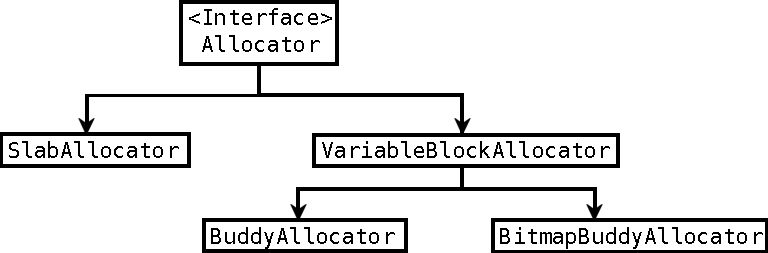
\includegraphics[width=0.8\textwidth]{images/allocator_interface_uml.pdf}
    \caption{Diagramma UML dell'interfaccia Allocator e delle sue implementazioni.}
    \label{fig:uml_allocator_interface}
\end{figure}

Le funzioni di cui manteniamo un riferimento all'interno delle \textit{struct} sono progettate per uso interno: infatti, gli argomenti sono passati attraverso modalità definite dalla libreria di sistema \texttt{<stdarg.h>}. In questo modo, possiamo mantenere i puntatori alle funzioni nonostante per le varie implementazioni della classe essi abbiamo \textit{signature} diverse, dando grande libertà e flessibilità. Contemporaneamente però questa pratica costituisce un rischio, poiché le verifiche sulla correttezza del tipo e del numero degli argomenti non sono fatte a \textit{compile-time}.

Per ovviare a questo problema e permettere al nostro programma di verificare correttamente che i parametri passati siano validi, introduciamo un buffer tra le funzioni interne e l’utente nella forma di funzioni helper segnalate come \textit{inline}. Attraverso esse, il programma mantiene la sua flessibilità internamente senza dover sacrificare in sicurezza: la correttezza dei parametri passati alla chiamata è effettuata dal compilatore e contemporaneamente la performance non è eccessivamente impattata da questo passaggio intermedio grazie alla keyword \textit{inline}. Essa indica al compilatore di ottimizzare aggressivamente la funzione, sostituendo alla chiamata il suo corpo (per questo motivo, è importante che queste funzioni helper siano brevi e concise, in modo da evitare \textit{code bloat}).

Una nota sulla keyword \textit{inline}: è importante ricordare che essa è un suggerimento e non un obbligo, per il compilatore: esistono modalità per forzare questa ottimizzazione, imponendo di applicarla a tutte le chiamate, ma questo potrebbe portare nel lungo termine a una minore ottimizzazione per via della quantità di codice, che renderebbe necessari più \textit{cache swaps} del necessario. Ulteriori test potrebbero mostrarne l’impatto e con ciò l’importanza di lasciare che sia il compilatore a occuparsi delle ottimizzazioni, ma ciò esula dagli scopi dell’analisi.

Ogni classe che implementa l’interfaccia \texttt{Allocator} deve implementare le proprie funzioni interne, che mantengono la stessa signature, e le funzioni \textit{wrapper}, che invece possono avere una signature diversa in base alle necessità. Per esempio, nell’allocazione di memoria per uno SlabAllocator (che velocemente anticipiamo poter allocare unicamente blocchi di memoria di grandezza omogenea) non sarà necessario specificare la grandezza dell’area richiesta. In più, deve fornire anche una rappresentazione grafica del suo stato ai fini di \textit{debugging} e analisi.

Le funzioni helper seguono una nomenclatura più vicina a quella della \textit{libc}, in modo da rendere l’API più intuitiva e immediata. Esse sono:
\begin{itemize}
    \item \texttt{Allocator\_create} (wrapper di \texttt{Allocator\_init})
    \item \texttt{Allocator\_destroy} (wrapper di \texttt{Allocator\_dest})
    \item \texttt{Allocator\_malloc} (wrapper di \texttt{Allocator\_reserve})
    \item \texttt{Allocator\_free} (wrapper di \texttt{Allocator\_release})
\end{itemize}
Per via del linker del linguaggio C, siamo costretti ad anteporre a nome della funzione la classe, come vediamo sopra. Sono state esplorate soluzioni a questo problema, ma sfortunatamente introducevano livelli di complessità oppure sacrificavano a livello di \textit{type checking}. Grazie alla duplice struttura con funzioni helper e internal sarebbe possibile realizzare in C una forma semplice di \textit{polimorfismo}, ma risulta sempre necessario, al netto dell’utilizzo di macro (che reintrodurrebbero i problemi evidenziati precedentemente), usare nomi univoci per ogni funzione con diversa combinazione di parametri.

\subsection{Richiesta iniziale di memoria}
Tutte le classi che implementano l’interfaccia \texttt{Allocator} usano \textit{mmap} per chiedere memoria al sistema operativo. Durante la fase di progetto, è stato valutato alternativamente di poter utilizzare la primitiva \textit{sbrk}, fornita dalla libreria C standard, che permette di “accrescere” l’\textit{heap} esplicitamente. Questo approccio avrebbe permesso un più granulare controllo sulla memoria al costo di una minore flessibilità e, dal punto di vista didattico, avrebbe costituito un'importante opportunità per studiare come avveniva l’allocazione di memoria in versioni precedenti della \textit{sbrk}.
Si è ritenuto tuttavia di usare \textit{mmap} per evitare complicazioni nella deallocazione (la memoria allocata attraverso \textit{sbrk} può infatti essere deallocata solamente in modo sequenziale o si rischia di introdurre frammentazione). La struttura a cui si può accedere attraverso \textit{sbrk} è infatti di tipo LIFO, ossia una pila di memoria. Ciò avrebbe potuto creare problemi laddove gestori fossero distrutti in ordine diverso da quello di creazione o si fosse deciso di permettere l’utilizzo \textit{multithreaded} \footnote{Al netto di possibili complicazioni impreviste, il supporto per l'utilizzo da parte di più entità potrebbe essere aggiunto con relativa facilità adoperando \textit{mutex} per contingentare le operazioni di richiesta e rilascio di memoria.}.

La flag \texttt{MAP\_ANONYMOUS} (anche nota come \texttt{MAP\_ANON}) è stata adoperata alla chiamata di \textit{mmap}. Essa fa sì che la memoria richiesta non sia “supportata” da alcun file. Dal manuale, “The mapping is not backed by any file; its contents are initialized to zero. The fd argument is ignored; however, some implementations require fd to be \texttt{-1}. If \texttt{MAP\_ANONYMOUS} (or \texttt{MAP\_ANON}) is specified, and portable applications ensure this. The offset argument should be zero. for \texttt{MAP\_ANONYMOUS} in conjunction with \texttt{MAP\_SHARED} added in Linux 2.4.” La memoria si trova dunque nella RAM fisica e non fa riferimento a un file \footnote{Chiaramente a meno che non sia stata posta in un file di swap}.

\begin{center}
\begin{tabular}{|l|l|l|}
\hline
Feature & \textit{sbrk} & \textit{mmap}(MAP\_ANONYMOUS) \\
\hline
Memory Type & Heap-only & Any virtual address \\
Fragmentation & High (contiguous heap) & Low (independent mappings) \\
Deallocation & Only last block & Arbitrary (\textit{munmap}) \\
File Backing & No & No (unless explicitly mapped) \\
Modern Usage & Legacy (brk in \textit{malloc}) & Preferred for large allocations \\
\hline
\end{tabular}
\end{center}

% TODO add section about massif and valgrind

\section{La classe SlabAllocator}
Lo \textit{slab allocator} è un gestore pensato per richieste di memoria di taglia costante. La sua struttura interna lo rende adatto quando sono necessarie unicamente allocazioni di memoria di dimensione nota e fissa (ad esempio, un'istanza di una classe): il termine \textit{slab} fa riferimento a questa “fetta” di memoria. Esso è dunque particolarmente efficiente al costo di flessibilità ridotta.

\begin{lstlisting}
struct SlabAllocator {
    Allocator base;
    char* managed_memory;
    unsigned int buffer_size;
    size_t slab_size;   
    size_t user_size;
    DoubleLinkedList* free_list;   
    unsigned int free_list_size;
    unsigned int free_list_size_max;
};
\end{lstlisting}

La prima menzione di un’implementazione di \textit{slab allocator} viene descritta nell’articolo di Jeff Bonwick \textit{“The Slab Allocator: An Object-Caching Kernel Memory Allocator”}~\cite{slab} del 1994. In esso vengono elencati i benefici di una soluzione che, rispetto a quella da noi implementata, risulta ben più complessa e strutturata. Il codice di Bonwick infatti trae beneficio non solo dalla taglia definita dei \textit{chunk}, ma anche dalla conoscenza della struttura dei dòati che verrà allocata nella memoria richiesta (dichiarata alla creazione del gestore). I blocchi liberi vengono già inizializzati come oggetti e mantengono la loro struttura alla restituzione del blocco, evitando così di dover spendere risorse per riorganizzare la memoria alla prossima richiesta. L’idea consiste nel “preservare la porzione invariante dello stato iniziale di un oggetto nell’intervallo tra gli usi, in modo che essa non debba essere distrutta e ricreata ogni volta che l’oggetto è usato.”

Non scendiamo ulteriormente nei dettagli del gestore di Bonwick per semplicità, ma notiamo che per quanto possa sembrare a posteriori non significativa, l’eleganza della sua soluzione è degna di nota. L’autore dell’articolo infatti non solo definisce algoritmi efficienti e con strumenti approfonditi per il \textit{debugging}, ma si cura di approfondire la relazione tra il suo algoritmo e le strutture del sistema operativo, in particolare con il \textit{Translation Lookaside Buffer}, fornendo chiare evidenze dell’attenzione posta non solo nell’approccio teorico, ma anche all’applicazione pratica del suo gestore. La specializzazione della soluzione applicata da Bonwick la rende ideale per l’utilizzo all’interno di sistemi operativi, che gestiscono spesso numerosi oggetti rappresentati da strutture dati di grandezza nota e fissa (\textit{socket}, \textit{semafori}, \textit{file}…). La prima implementazione di questo modello è presentata nel kernel di SunOS 5.4, per poi comparire a uso interno a molti altri kernel, compreso quello di FreeBSD (v5.0) e Linux (a partire dalla versione 2.1.23), dove successivamente diventerà anche disponibile per l’uso da parte dell’utente.

Nella nostra implementazione non viene fatto \textit{caching} della struttura interna dell’oggetto e l’utente è lasciato libero di gestire liberamente lo slab assegnato. Chiaramente, questo lo rende ordini di grandezza più lento della soluzione applicata da Bonwick. Lo scopo didattico nonostante questo è la dimostrazione di come l’efficienza dei gestori dinamici di memoria sia strettamente correlata alla comprensione da parte del programmatore delle richieste fatte durante il corso della vita dell’applicazione: lo \textit{slab allocator} può essere usato al massimo delle sue potenzialità solo a seguito della profonda comprensione del succedersi delle allocazioni e rilasci di memoria.

\subsection*{Funzionamento dello SlabAllocator}
Come stabilito precedentemente, l’utente non usa le funzioni interne per accedere alle funzionalità del gestore, ma bensì adopera i metodi helper sotto delineati, la cui funzione è puramente quella di "filtro" a tempo di compilazione dei parametri e di gestire in maniera appropriata il valore di ritorno delle funzioni interne

\begin{lstlisting}
inline SlabAllocator* SlabAllocator_create(SlabAllocator* a, size_t slab_size, size_t n_slabs);
inline int SlabAllocator_destroy(SlabAllocator* a);
inline void* SlabAllocator_malloc(SlabAllocator* a);
inline int SlabAllocator_free(SlabAllocator* a, void* ptr);
\end{lstlisting}

L’inizializzazione di un’istanza di SlabAllocator richiede la grandezza dello slab (nei termini di Bonwick, la grandezza dell’oggetto da immagazzinare) e il numero delle stesse. Dopo una serie di controlli sui parametri, la memoria richiesta viene suddivisa in blocchi. Essi sono dunque organizzati in una \textit{linked list}, che mantiene un pratico riferimento alla memoria disponibile e la cui lunghezza massima è pari al numero totale di blocchi. Al termine dell’uso le operazioni di distruzione sono immediate: l’unica accortezza è restituire la memoria al sistema operativo con \textit{unmap}.

\begin{figure}[H]
    \centering
    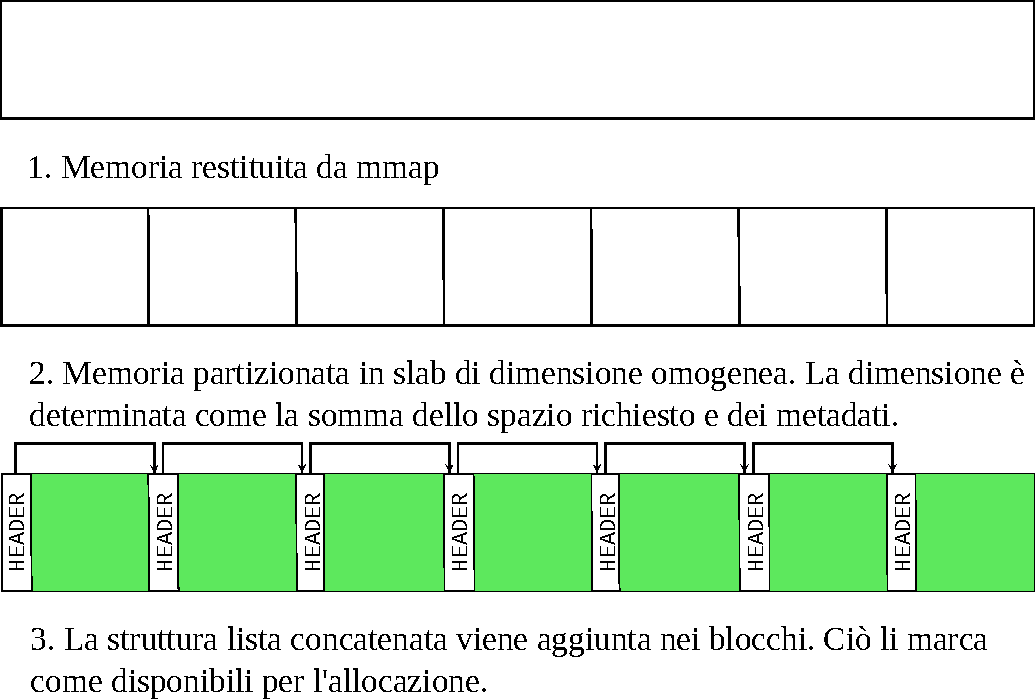
\includegraphics[width=0.8\textwidth]{images/slab/slab_allocator_init.pdf}
    \caption{Inizializzazione dello SlabAllocator: suddivisione della memoria in blocchi di dimensione fissa e organizzazione in una lista concatenata.}
    \label{fig:slab_allocator_init}
\end{figure}

Lo spazio per gestire l’appartenenza del blocco alla lista (ossia i campi di SlabNode, sottoclasse di Node) sono inseriti in cima al blocco. Ciò rende la struttura manipolabile da parte dell’utente, che può inavvertitamente o con intenzioni maligne corromperli scrivendo sopra di essi. A questa problematica sarebbe possibile porre rimedio mantenendo in memoria una struttura dati che tenga un riferimento di tutti gli indirizzi allocati e li possa dunque verificare. Tuttavia, ciò introdurrebbe complicazioni e la scelta implementativa di “fidarsi dell’utente” ricalca quella che è stata adottata nella libc con \textit{malloc}.

Poiché tutti i blocchi hanno la stessa dimensione, alla richiesta non è necessario stabilire quale di essi sia più opportuno allocare: la suddivisione avviene a priori durante l’inizializzazione del gestore, e la taglia dei blocchi non è modificata in nessun momento. La lista viene consultata e il blocco in testa viene estratto e restituito. Quando un blocco viene rilasciato, l’indirizzo di memoria viene controllato: se esso risulta essere corretto, viene semplicemente inserito al primo posto della lista per uso futuro. Notiamo che l’ordine della lista non rappresenta assolutamente la contiguità dei blocchi e richieste immediatamente successive possono ritornare blocchi non contigui.

\subsection*{Efficienza dello SlabAllocator}
Descriviamo ora più nel dettaglio la complessità computazionale delle operazioni compiute dal gestore. L’allocazione ha un costo costante, così come la liberazione di un blocco, poiché in entrambi i casi viene semplicemente manipolata la testa di una \textit{linked list} contenente i riferimenti ai blocchi liberi. I blocchi non sono in alcun modo manipolati: la loro grandezza rimane costante e questo elimina completamente i costi legati alle operazioni di divisione e unione.

Grazie alla sua struttura particolare, lo \textit{slab allocator} non può mai presentare frammentazione esterna: poiché tutti i blocchi hanno la stessa dimensione, se è presente almeno uno slab di memoria libero, la richiesta dell’utente potrà essere esaudita e non può mai esistere memoria libera che l’utente non può chiedere di utilizzare. La frammentazione interna viene invece limitata dal programmatore, che, conoscendo le proprie necessità, può scegliere all’inizializzazione del gestore la dimensione del blocco più appropriata per i propri scopi.

\begin{center}
\begin{tabular}{|l|l|}
\hline
Operazione & SlabAllocator \\
\hline
Allocazione & $O(1)$ \\
Deallocazione & $O(1)$ \\
Ricerca blocco libero & $O(1)$ \\
Frammentazione interna & Determinata dal programmatore all'inizializzazione \\
Frammentazione esterna & Nulla \\
\hline
\end{tabular}
\end{center}

L’efficienza dello \textit{slab allocator} dipende quindi dalla corretta scelta iniziale della dimensione dei blocchi. Tuttavia, in scenari dove le esigenze variano nel tempo (ossia si rende necessaria l’allocazione di oggetti di taglia diversa) è possibile combinare più gestori slab, ciascuno ottimizzato per una diversa dimensione. Questo approccio ibrido mantiene i vantaggi della complessità costante per le operazioni base, introducendo un trade-off legato alla gestione di più liste separate. La frammentazione interna rimane comunque controllabile, poiché limitata alla discrepanza tra la dimensione richiesta e quella dello slab più adatto.

Abbiamo già definito come, nel caso sia nota la dimensione massima necessaria per un blocco di memoria, lo \textit{slab allocator} sia molto efficiente. Tuttavia, si potrebbero presentare situazioni in cui gli slab completamente liberi occupano memoria inutilmente, perché ad esempio il numero di \textit{chunk} è molto maggiore di quello degli oggetti che contemporaneamente vengono allocati. La necessità di slab del programma potrebbe variare nel corso delle operazioni da esso svolte. Per mitigare questo problema, alcune implementazioni introducono meccanismi di \textit{reclaiming}: dopo un periodo di inattività o sotto pressione di memoria, gli slab vuoti possono essere rilasciati al sistema operativo. Questa operazione, seppur con un costo aggiuntivo (tipicamente $O(n)$ rispetto al numero di slab liberi), è compensata dalla flessibilità nel ridurre l’impronta memoria quando necessario. Per la nostra applicazione ciò non è stato ritenuto necessario.

Rispetto a gestori generici (come \textit{buddy system} o \textit{malloc} tradizionale), lo \textit{slab allocator} eccelle in velocità e assenza di frammentazione esterna, ma è meno adatto a contesti con richieste eterogenee. La sua complessità spaziale è proporzionale al numero di slab preallocati, il che lo rende ideale per sistemi con risorse dedicate e pattern di allocazione prevedibili.

\section{La classe BuddyAllocator}
Il problema dell’allocazione di memoria per richieste di dimensioni variabili rimane un tema aperto e ampiamente discusso. Diversi approcci alla sua soluzione sono stati discussi nel tempo, suscitando dibattiti e proposte contrastanti. Sono state sviluppate numerose alternative, ciascuna con i propri vantaggi e limiti, ottenendo livelli di adozione e consenso variabili nell'ambito dei sistemi moderni.

I primi tentativi alla divisione dinamica dello spazio disponibile presero il nome di \textit{“sequential fits”}. In base alle necessità e richieste del programma in esecuzione, la memoria viene divisa in blocchi di dimensione variabile. Essi, organizzati in un'unica lista concatenata, sono esplorati con costo lineare per trovare il first (il primo blocco sufficientemente grande) o best fit (il blocco più piccolo in grado di soddisfare la richiesta).

Questa soluzione, famosamente esplorata da Knuth, presenta importanti limitazioni. La perdità di scalabilità per via del costo lineare è un punto critico: all’aumentare del numero di blocchi, il costo temporale della ricerca diventa proibitivo. Sebbene con dovuti accorgimenti si possano evitare un eccessivo overhead e una debilitante frammentazione\footnote{Knuth stesso ne ha proposto uno che successivamente è diventato molto popolare: il concetto di \textit{boundary tag}, ossia salvare le informazioni al termine dell'area allocata per facilitare la riunione dei blocchi.}, l’inefficienza della scansione lineare è il fattore che principalmente ne impedisce l'applicazione nei contesti ad alte prestazioni.

L’evoluzione di questo algoritmo mantiene la divisione dinamica in taglie non prestabilite, ma prova a risolvere il problema della lunghezza eccessiva della lista: investire nell’organizzazione maggiore spazio, gestendo i blocchi liberi più efficientemente, permette di velocizzare la ricerca del blocco corretto. La memoria disponibile viene suddivisa sempre in blocchi liberi, che sono però raccolti in base alla loro taglia in liste diversificate. La struttura è semplice e simile a quella del metodo visto precedentemente, tuttavia grazie alla lunghezza minore delle singolari liste, esse sono più rapidamente esplorabili.

Al momento della richiesta, è esaminata la lista contenente i blocchi della taglia più appropriata, e laddove non vi sia un blocco adeguato vengono ricorsivamente controllate le liste di livello "superiore", contenente blocchi di dimensione maggiore. Il blocco eventualmente individuato è suddiviso e la memoria in eccesso (quella che non risulta necessaria per soddisfare la richiesta di memoria) è organizzata in un nuovo \textit{chunk} libero che viene riposto nella lista corretta secondo la sua grandezza. Questo meccanismo viene chiamato nell’articolo di Wilson et al. \textit{“segregated free lists”}.

Il \textit{Buddy Allocator} è descritto nella stessa pubblicazione come un “caso particolare” di quest'ultima tipologia di allocatori. Inventato da Harry Markowitz nel 1963 e pubblicato per la prima volta nell’articolo \textit{“A Fast Storage Allocator”}~\cite{knowlton1965} del 1965 da Kenneth C. Knowlton, ingegnere presso Bell Telephone Laboratories, il \textit{buddy system} è facile da implementare e presenta buoni risultati se usato in risposta a richieste di taglia variabile, ma generalmente nota, che vengono ripetute numerose volte.
 
La differenza rispetto agli algoritmi che lo precedono consiste principalmente nelle politiche di \textit{splitting} e \textit{coalescing}. Se la metodologia descritta nel paragrafo precedente non stabilisce esplicitamente se, come o quando i blocchi liberi debbano essere riuniti e aggiunti alle \textit{free lists} di grandezza maggiore, i \textit{buddy systems} invece stabiliscono una chiara gerarchia che rende il procedimento più ordinato. I blocchi infatti, come approfondiremo successivamente, sono infatti partizionati sempre secondo le stesse modalità in metà uguali.

Questa differenza consente di evitare un problema significativo che emerge quando la dimensione dei blocchi non è vincolata. In particolare, modelli di allocazione tipici, come l'alternanza di richieste e rilasci di blocchi di dimensioni diverse, causano frammentazione esterna negli allocatori che adottano metodi come i \textit{sequential fits}. La libertà nella gestione delle dimensioni dei blocchi unita alla ricerca lineare porta alla formazione di numerose aree libere sparse e non contigue. Gli allocatori con \textit{segregated free lists}, sebbene più efficienti grazie alla suddivisione in liste separate per intervalli di dimensione, non sono immuni al problema.

Il \textit{Buddy Allocator} rappresenta una soluzione elegante al problema della frammentazione esterna grazie alla sua struttura costituita da blocchi le cui dimensioni sono esclusivamente potenze di due. Ciò previene la formazione di aree di memoria inutilizzabili e garantisce che tutti i blocchi allocati abbiano dimensioni standardizzate.

\subsection*{Funzionamento del BuddyAllocator}
Ogni blocco di memoria è rappresentato da un BuddyNode, che contiene metadati come la dimensione, un’indicazione sullo stato e puntatori al buddy e al parent. La scelta di memorizzare esplicitamente queste relazioni, anziché calcolarle dinamicamente attraverso manipolazione degli indirizzi di memoria, semplifica il debug e la visualizzazione dello stato dell'allocatore: infatti, poiché sono note la taglia del blocco e l’indirizzo di partenza, gli header del buddy e del parent potrebbero essere raggiunti senza bisogno di immagazzinare esplicitamente questa informazione nell’header.

\begin{lstlisting}
typedef struct BuddyNode {
    Node node;
    char *data;
    size_t size;                // Size of this block (including header)
    int level;                  // Level in the buddy system
    int is_free;                // Whether this block is free
    struct BuddyNode* buddy;    // Pointer to buddy block
    struct BuddyNode* parent;   // Pointer to parent block
} BuddyNode;
\end{lstlisting}

I nodi non sono salvati in una struttura ad albero, ma bensì in una serie di free lists, corrispondenti ai vari livelli dello stesso. La metodologia è ripresa dalle tecniche elencate precedentemente negli algoritmi “segregated free lists”. Alla creazione, viene richiesto all’utente la grandezza dell’area di memoria da gestire e il numero massimo di livelli (alternativamente, poteva essere richiesta la grandezza del blocco di dimensione minima). L'allocatore utilizza due SlabAllocator interni: uno per gestire i BuddyNode e l'altro per le liste libere, che vengono tutte inizializzate alla creazione. Questa scelta rappresenta un chiaro luogo dove le caratteristiche dello slab allocator possano essere valorizzate, poiché le dimensioni degli oggetti allocati sono fisse e note a priori.

\begin{lstlisting}
typedef struct BuddyAllocator {
    Allocator base;           // Base allocator interface
    void* memory_start;       // Start of managed memory
    size_t total_size;        // Total size of managed memory
    size_t min_block_size;    // Minimum block size (power of 2)
    int num_levels;           // Number of levels in the system
    SlabAllocator list_allocator;
    SlabAllocator node_allocator;
    DoubleLinkedList* free_lists[BUDDY_MAX_LEVELS];  // Array of free lists for each level
} BuddyAllocator;
\end{lstlisting}

Dalla descrizione del sistema buddy, notiamo facilmente che la struttura dati delineata corrisponde a un albero binario. Infatti, ogni nodo (blocco di memoria) tranne la radice possiede un singolo genitore e un buddy. Esso può inoltre a sua volta essere scomposto in ulteriori due nodi liberi. Un vantaggio della struttura binaria è che il buddy corrisponde sempre con il blocco adiacente (precedente o successivo).

\begin{lstlisting}
inline BuddyAllocator* BuddyAllocator_create(BuddyAllocator* a, size_t total_size, int num_levels);
inline int BuddyAllocator_destroy(BuddyAllocator* a);
inline void* BuddyAllocator_malloc(BuddyAllocator* a, size_t size);
inline int BuddyAllocator_free(BuddyAllocator* a, void* ptr);
\end{lstlisting}

Quando è necessario dividere un blocco per soddisfare una richiesta, esso viene diviso in parti uguali e i blocchi ottenuti diventano buddies, aventi chiaramente la stessa dimensione. Al rilascio da parte dell’utente, il blocco controlla il suo buddy e verifica se esso sia a sua volta libero. Nell’eventualità che entrambi i buddies siano contemporaneamente non riservati dall’utente, essi vengono riunificati nel blocco parent da cui derivano. Sia l'operazione di divisione dei blocchi che quella di ricongiungimento sono svolte in modo ricorsivo, esplorando tutti i livelli dell'albero fino a che la richiesta non sia stata esaudita o sia stato accertato che non vi siano blocchi liberi per farlo. 

\subsection*{Efficienza del BuddyAllocator}
L’architettura del buddy system risolve radicalmente il problema della frammentazione esterna tipica degli allocatori tradizionali. La memoria libera viene infatti divisa equamente in base alle necessità reali del programma e costantemente riaggregata in blocchi ordinati e perfettamente allineati. Tuttavia, questa soluzione non è esente da compromessi. L'arrotondamento sistematico alla potenza di due superiore comporta inevitabilmente una certa quantità di frammentazione interna, particolarmente evidente quando le richieste di memoria sono solo leggermente superiori a una data potenza di due. Inoltre, la rigidità del sistema lo rende meno adatto a gestire pattern di allocazione estremamente variabili o imprevedibili.

L'operazione di allocazione cerca prima nella lista libera del livello appropriato. Se non trova blocchi disponibili, risale ai livelli superiori, dividendo i blocchi fino a raggiungere la dimensione desiderata. Questo approccio garantisce un costo $O(1)$ nel caso ideale (blocco disponibile nel livello corretto) e $O(L)$ nel caso peggiore, dove L è il numero di livelli. La fusione dei blocchi liberi avviene in tempo $O(L)$, grazie alla verifica ricorsiva dello stato del buddy.

L'uso di free lists separate per ogni livello elimina la necessità di strutture ad albero complesse, semplificando l'implementazione e riducendo l'overhead. Tuttavia, l'allocatore paga un costo in termini di memoria per i metadati aggiuntivi (puntatori a buddy e parent), che potrebbe essere evitato con un calcolo dinamico degli indirizzi dei buddy. La tecnica adoperata nel BuddyAllocator evita frammentazione esterna, ma rischia di introdurne interna.

\begin{center}
\begin{tabular}{|l|l|}
\hline
Operazione & BuddyAllocator \\
\hline
Allocazione & $O(1)$ / $O(L)$ \\
Deallocazione & $O(1)$ \\
Ricerca blocco libero & $O(1)$ / $O(L)$ \\
Frammentazione interna & Potenzialmente molto alta \\
Frammentazione esterna & Generalmente bassa \\
\hline
\end{tabular}
\end{center}

\section{La classe BitmapBuddyAllocator}
Nelle implementazioni analizzate finora, la ricerca di un blocco libero avviene tramite l'esplorazione di liste concatenate. Se queste sono correttamente ordinate o suddivise per dimensione, la scansione può essere relativamente efficiente quando il blocco cercato è presente. Tuttavia, un problema intrinseco di questo approccio è la possibile discontiguità spaziale dei blocchi nella lista, che può essere causa di inefficienza nella gestione della cache, causando numerosi miss.

Per ovviare a questa limitazione, sono stati introdotti allocatori che utilizzano strutture dati più avanzate per memorizzare le informazioni sui blocchi liberi, migliorando così l’efficienza grazie a un utilizzo della cache più avveduto. Essi nell’articolo di Wilson prendono il nome di \textit{"indexed fit"}. Tra le strutture usate, alberi binari bilanciati (\textit{self-balancing binary trees}) e \textit{heap} si sono dimostrati particolarmente efficaci; ciononostante, essi richiedono un costo gestionale non trascurabile per mantenere l’equilibrio della struttura.

Un approccio alternativo e più semplice rispetto alle strutture dati complesse è l’utilizzo di \textit{bitmap}: questa struttura dati, nota anche come \textit{bit array} o \textit{bit field}, permette di immagazzinare informazioni in modo denso e compatto.  Nella gestione del \textit{BitmapBuddyAllocator}, è fatto uso di una \textit{bitmap} dove ogni bit rappresenta lo stato, libero o occupato, del corrispondente blocco di memoria. A differenza delle liste concatenate (che richiedono dereferenziamenti di puntatori potenzialmente dispersi in memoria, con conseguenti \textit{cache miss}), le bitmap permettono di verificare lo stato dei blocchi in modo più efficiente, poiché le informazioni risiedono in memoria contigua. Ciò può anche avvalersi delle istruzioni SIMD (Single Instruction, Multiple Data) e funzionalità hardware avanzate fornite dall’architettura.

Si rende dunque necessario mitigare gli effetti della scansione mediante euristiche che restringono l’area di esplorazione a intervalli predefiniti. In questo contesto, il buddy system visto nella sezione precedente riemerge come soluzione particolarmente efficace. Grazie alla sua struttura gerarchica binaria, esso permette infatti di individuare rapidamente i blocchi liberi e le relazioni tra di essi, ottimizzando sia l’allocazione che la deallocazione. In particolare, sfruttando una bitmap associativa, è possibile delimitare con precisione la zona di memoria in cui cercare i blocchi disponibili, migliorando ulteriormente l’efficienza.

\subsection*{Funzionamento del BitmapBuddyAllocator}
La memoria necessaria per gestire la bitmap viene gestita all'interno dell'area assegnata all'allocatore dall'operazione di \textit{mmap}

\begin{lstlisting}
inline BitmapBuddyAllocator* BitmapBuddyAllocator_create(BitmapBuddyAllocator* a, size_t total_size, int num_levels);
inline int BitmapBuddyAllocator_destroy(BitmapBuddyAllocator* a);
inline void* BitmapBuddyAllocator_malloc(BitmapBuddyAllocator* a, size_t size);
inline int BitmapBuddyAllocator_free(BitmapBuddyAllocator* a, void* ptr);
\end{lstlisting}

Poiché il BitmapBuddyAllocator è una variante del classico buddy system, le operazioni che esso svolge sono simili a quelle viste precedentemente: la differenza è nella struttura dati che viene consultata. (la bitmap piuttosto delle liste concatenate). Quando viene richiesta della memoria, l’allocatore cerca nella bitmap un blocco libero della dimensione giusta. Se non lo trova, risale di livello per trovarne uno più grande e lo suddivide nei due buddy di dimensione uguale, aggiornando la bitmap di conseguenza. Un blocco parent che sia scomposto in buddy di cui almeno uno è utilizzato è segnato a sua volta come non adoperabile per esaudire richieste, in quanto parte di esso è allocata.

\begin{lstlisting}
// Returns the level in the binary tree for a given index.
// Formula: level = floor(log2(idx + 1))
static int levelIdx(size_t idx) {
    return (int)floor(log2(idx+1));
}

// Returns the buddy index for a given node index.
// Formula: buddyIdx = idx - 1 if idx is odd, idx + 1 if idx is even (except root)
// buddyIdx = idx ^ 1 (bitwise alternative)
static int buddyIdx(int idx) {
    if (idx == 0) return 0;
    return idx % 2 ? idx - 1 : idx + 1;
}

// Returns the parent index for a given node index.
// Formula: parentIdx = floor((idx - 1) / 2)
static int parentIdx(int idx) {
    return (idx - 1) / 2;
}

// Returns the first index at a given level in the binary tree.
// Formula: firstIdx = 2^level - 1
static int firstIdx(int level) {
    return (1 << level) - 1;
}

// Returns the position of idx within its level.
// Formula: startIdx = idx - firstIdx(level)
// Returns -1 if level is invalid (>= num_levels)
static int startIdx(int idx, int num_levels) {
    int level = levelIdx(idx);
    if (level >= num_levels) return -1;  // Invalid level
    return idx - firstIdx(level);
}
\end{lstlisting}

Durante la deallocazione, il bit del blocco viene segnato come libero. Se anche il buddy è libero, i due vengono fusi e il blocco originario viene ricostruito, riducendo la frammentazione. In breve, il BitmapBuddyAllocator unisce la flessibilità del buddy system con la velocità e compattezza delle bitmap, risultando ideale per ambienti ad alte prestazioni.

\subsection*{Efficienza del BitmapBuddyAllocator}
Il BitmapBuddyAllocator rappresenta un compromesso ottimale tra efficienza (grazie alle ottimizzazioni bitwise), semplicità (nessuna gestione di strutture complesse come alberi bilanciati) e scalabilità (adatto a sistemi con grandi pool di memoria). Mentre il BuddyAllocator tradizionale rimane una scelta valida in contesti semplici, in quanto di più facile implementazione, il BitmapBuddyAllocator si dimostra superiore in scenari ad alte prestazioni, dove è critico il ruolo del caching. 

Questo metodo consente una ricerca estremamente rapida di blocchi contigui liberi, migliorando significativamente la località spaziale e riducendo i problemi di caching tipici delle liste. Tuttavia, poiché la verifica della disponibilità richiede comunque l’ispezione sequenziale dei bit (seppur accelerata da ottimizzazioni hardware), la complessità computazionale rimane $O(n)$ per algoritmi come first-fit o best-fit. Tuttavia, la frammentazione interna rimane un problema irrisolto, rendendo questo allocatore meno adatto per carichi di lavoro con richieste di memoria estremamente variabili.

\begin{center}
\begin{tabular}{|l|l|}
\hline
Operazione & BitmapBuddyAllocator \\
\hline
Allocazione & $O(1)$ / $O(L)$ \\
Deallocazione & $O(1)$ \\
Ricerca blocco libero & $O(1)$ / $O(L)$ \\
Frammentazione interna & Potenzialmente molto alta \\
Frammentazione esterna & Generalmente bassa \\
\hline
\end{tabular}
\end{center}


\chapter[Test e Performance]{Test e Performance}

La letteratura descritta nel secondo capitolo giunge a una conclusione concorde sui benchmark per i gestori di memoria dinamicamente allocata: per valutare un algoritmo di allocazione, è necessario osservarne il comportamento all’interno di un contesto realistico. Ciò può avvenire solamente laddove le tracce adoperate per condurre i benchmark siano vicine alle allocazioni realmente compiute da programmi reali, che sono presi come esempio (esistono utilities che permettono di registrare le richieste, in modo da poterle usare a questo scopo).

Quando le tracce sono casualmente generate, il risultato finale ci dice ben poco sulle capacità effettive dell’allocatore. Le richieste prodotte da un algoritmo probabilistico creano un modello di comportamento, ma questo non è sufficiente: riprodurre le complesse interazioni tra allocazioni e deallocazioni di memoria è molto difficile, poiché queste ultime sono poco comprese e differiscono grandemente tra tipologie di applicazione. Il comportamento a fasi dei programmi dà vita a fenomeni di interconnessione sistematica che sono per la maggior parte ignorati.

Nel 1998, Wilson e Johnston approfondiscono i risultati del procedente paper sull’allocazione dinamica di memoria indagando il comportamento di diversi noti programmi scritti in C e C++. Nell’articolo \emph{The Memory Fragmentation Problem: Solved?}~\cite{wilson1998} gli autori tentano di dimostrare come la frammentazione può essere evitata laddove sia scelta con attenzione una politica di allocazione appropriata a prescindere dall’implementazione.

\begin{quote}
``This substantially strengthens our previous results showing that the memory fragmentation problem has generally been misunderstood, and that good allocator policies can provide good memory usage for most programs. The new results indicate that for most programs, excellent allocator policies are readily available, and efficiency of implementation is the major challenge.''

\begin{center}
[...]
\end{center}

``If these results hold up to further study with additional programs, we arrive at the conclusion that the fragmentation problem is a problem of recognizing that good allocation policies already exist, and have inexpensive implementations. For most programs, the problem of simple overheads is more significant than the problem of fragmentation itself.''
\end{quote} 

Il programma è stato sottoposto anche ad analisi attraverso \textit{valgrind}, il popolare programma di \textit{debugging} e \textit{memory analysis}, in particolare adoperando i \textit{tool} \textit{memcheck, massif} e \textit{cachegrind}. Questi strumenti sono stati fondamentali per comprendere in primo luogo se il programma accedesse alla memoria come previsto, e secondariamente per comprendere dove si trovassero le ostruzioni e i punti critici che causavano perdita di efficienza.

\section{Test delle funzionalità}

I test delle funzionalità si concentrano unicamente sulla correttezza del codice: verificano che le funzioni rispondano correttamente a parametri sbagliati o richieste inappropriate. Definendo la flag \lstinline|DEBUG| a tempo di compilazione abbiamo accesso a maggiori informazioni sugli errori e sulle loro cause. 

\subsection{SlabAllocator}
\begin{table}[H]
\centering
\begin{tabularx}{\textwidth}{|l|X|}
\hline
\textbf{Nome del Test} & \textbf{Descrizione} \\
\hline
\texttt{test\_invalid\_init} & Verifica che l'allocatore gestisca correttamente parametri di inizializzazione non validi (es. dimensione zero o numero massimo di slab non valido). \\
\hline
\texttt{test\_create\_destroy} & Controlla che la creazione e distruzione di uno slab avvengano correttamente, senza memory leak o errori. \\
\hline
\texttt{test\_alloc\_pattern} & Testa il comportamento dell'allocatore con un pattern di allocazioni e deallocazioni ripetute per verificare la correttezza della gestione della memoria. \\
\hline
\texttt{test\_exhaustion} & Verifica il comportamento quando lo slab è pieno (es. ritorno di NULL o gestione degli errori quando non c'è più memoria disponibile). \\
\hline
\texttt{test\_invalid\_free} & Controlla come l'allocatore gestisce la deallocazione di puntatori non validi (es. NULL o indirizzi non allocati). \\
\hline
\end{tabularx}
\caption{Test funzionali per SlabAllocator}
\end{table}

I test per lo SlabAllocator sono generalmente semplici in natura: poiché la grandezza della richiesta non varia e la lista da gestire è singola, gli unici punti di difficoltà sono la creazione con parametri invalidi o il rilascio di puntatori incorretti.


\subsection{BuddyAllocator e BitmapBuddyAllocator}
\begin{table}[H]
\centering
\begin{tabularx}{\textwidth}{|l|X|}
\hline
\textbf{Nome del Test} & \textbf{Descrizione} \\
\hline
\texttt{test\_invalid\_init} & Verifica che l'allocatore gestisca correttamente inizializzazioni non valide (es. dimensione zero, parametri NULL, o valori non supportati). \\
\hline
\texttt{test\_create\_destroy} & Testa la corretta creazione e distruzione di un allocatore, assicurandosi che non ci siano memory leak o corruzione dei dati. \\
\hline
\texttt{test\_single\_allocation} & Verifica che l'allocatore possa rispondere correttamente ad allocazioni invalide e gestire correttamente una singola allocazione. \\
\hline
\texttt{test\_multiple\_allocation} & Controlla il comportamento dell'allocatore quando vengono effettuate più allocazioni consecutive, assicurandosi che tutte abbiano successo e non si sovrappongano. \\
\hline
\texttt{test\_varied\_sizes} & Testa l'allocazione di blocchi di dimensioni diverse per verificare che l'allocatore gestisca correttamente richieste eterogenee. \\
\hline
\texttt{test\_buddy\_merging} & Verifica che, dopo una serie di allocazioni e deallocazioni, l'allocatore riesca a fondere correttamente i blocchi liberi adiacenti (buddy merging) per evitare frammentazione. \\
\hline
\texttt{test\_invalid\_reference} & Controlla come l'allocatore gestisce tentativi di deallocazione di riferimenti non validi (es. NULL, doppio free, o puntatori non allocati). \\
\hline
\end{tabularx}
\caption{Test funzionali per BuddyAllocator e BitmapBuddyAllocator}
\end{table}

Gli allocatori che accettano richieste a taglia variabile presentano una complessità maggiore rispetto a quelli a taglia fissa, poiché devono gestire dinamicamente la suddivisione e la fusione dei blocchi di memoria per rispondere a richieste di dimensioni differenti. Questo comporta una maggiore probabilità di introdurre errori nella gestione della memoria come la perdita di riferimenti o la mancata fusione dei blocchi liberi (\emph{buddy merging}). I test svolgono un ruolo fondamentale nell'evidenziare anomalie e comportamenti indesiderati

Oltre ai test elencati, è utile prevedere casi limite e scenari di stress, come sequenze di allocazioni e deallocazioni ripetute con dimensioni variabili, tentativi di allocazione che saturano la memoria disponibile, e la verifica della corretta gestione di errori (ad esempio, \emph{double free} o allocazioni fuori dai limiti consentiti).

\section{Benchmark}
Poiché la nostra analisi si concentra principalmente sulla correttezza dell'implementazione, i test sopra delineati forniscono una prima conferma del nostro operato. Tuttavia, l'importanza della \textit{performance} dell'allocatore in diversi casi applicativi risulta essenziale per poter veramente trarre delle conclusioni a riguardo. 
Nel corso delle ricerche, l'articolo \textit{"Designing a Trace Format for Heap Allocation Events"}~\cite{chilimbi2000} di T.Chilimbi et al ha fornito un'interessante base teorica per il parser qui descritto. Tuttavia, il nostro vuole essere unicamente un prototipo di funzionamento al fine di svolgere analisi più profonde, e sicuramente fornisce ben poche delle capacità descritte nell'articolo o altrimenti rese disponibili da altri strumenti simili applicati nel campo.\footnotemark

\footnotetext{Alcuni di questi che menzioniamo per dovere di cronaca sono \texttt{perf, LTTng} e \texttt{ETW}. }

Per facilitare dunque l’analisi del comportamento degli allocatori in presenza di pattern complessi di allocazione e deallocazione, è stata introdotta una funzionalità che consente di definire facilmente le sequenze di richieste di memoria tramite file di configurazione esterni, senza dover modificare o ricompilare il codice sorgente. In questo modo è possibile variare rapidamente i benchmark e testare diversi scenari. Il codice sorgente di questa funzionalità si trova nei moduli \texttt{benchmark} e \texttt{parse}.

Ciò è reso possibile dall’implementazione da parte di ogni allocatore dell’interfaccia \texttt{<Allocator>}. Poiché abbiamo a nostra disposizione i puntatori alle funzioni necessarie per svolgere tutte le operazioni, possiamo standardizzare il funzionamento delle classi dividendole in due categorie: allocatori a taglia fissa, che permettono di richiedere blocchi di grandezza prestabilita (e.g. \texttt{SlabAllocator}) e allocatori a taglia variabile, ossia le classi "figlie" di \texttt{VariableBlockAllocator}, le quali invece lasciano all’utente la scelta della dimensione dell’area di memoria richiesta (ossia \texttt{BuddyAllocator} e \texttt{BitmapBuddyAllocator}, nella nostra implementazione).

\begin{lstlisting}
  // template per allocatore a dimensione fissa
  void *FixedSizeAllocator_malloc(FixedSizeAllocator *a);
  void *FixedSizeAllocator_free(FixedSizeAllocator *a);
  // template per allocatore a dimensione variabile
  void *VariableSizeAllocator_malloc(VariableSizeAllocator *a, size_t size);
  void *VariableSizeAllocator_free(VariableSizeAllocator *a)
\end{lstlisting}

Il programma cerca all’interno della cartella \texttt{./benchmarks} file che abbiano l’estensione \texttt{.alloc}. Modificando il testo al loro interno si possono definire la tipologia di allocatore, i suoi parametri di inizializzazione e la sequenza di \texttt{malloc}/\texttt{free} da provare. I comandi sono terminati dal carattere ``a capo'' (\textbackslash n) e le componenti sono divise da una virgola. Comandi che sono preceduti dal carattere percentuale (\%) sono considerati commenti e ignorati.

Vediamo ora come descrivere la classe di allocatore da sottoporre al benchmark e le sue caratteristiche. La prima riga non preceduta da un segno percentuale deve avere necessariamente la seguente struttura: \texttt{i,<allocator class>} dove la classe può essere \texttt{slab}, \texttt{buddy} o \texttt{bitmap}. Il secondo comando informa il programma sui parametri di creazione: \texttt{p,<param1>,<param2>,\ldots}, il numero e il tipo dei quali varia in base alla classe scelta precedentemente.

\begin{table}[H]
\centering
\begin{tabularx}{\textwidth}{|X|X|X|X|}
\hline
\textbf{Allocatore} & \textbf{Dimensione} & \textbf{Parametro 1} & \textbf{Parametro 2} \\
\hline
Slab    & Fissa     & \texttt{slab\_size}   & \texttt{num\_slabs}   \\
\hline
Buddy   & Variabile & \texttt{memory\_size} & \texttt{max\_levels}  \\
\hline
Bitmap  & Variabile & \texttt{memory\_size} & \texttt{max\_levels}  \\
\hline
\end{tabularx}
\caption{Parametri di inizializzazione per ciascuna classe di allocatore}
\end{table}

Per allocare e liberare memoria, l’istruzione deve iniziare rispettivamente con ``a'' o ``f''. Il benchmark per tenere traccia delle allocazioni usa un array avente lunghezza pari al numero massimo possibile di frammenti di memoria. Il comando \texttt{a,<index>} alloca memoria in una posizione specifica dell'array, mentre \texttt{f,<index>} la libera. Nel caso di allocatore a richiesta variabile, dopo l’index dell’array va specificato il numero di byte da allocare (con struttura \texttt{a,<index>,<size>}). 

È fondamentale non allocare più volte sullo stesso indice senza prima liberarlo, altrimenti si perderà il riferimento all'area di memoria e non sarà più possibile gestirla correttamente\footnotemark. Il programma esegue la sequenza di \textit{request} e \textit{release}, informa l'utente di eventuali errori e stampa a schermo informazioni sul tempo richiesto: \texttt{elapsed\_seconds}, \texttt{user\_seconds} e \texttt{kernel\_seconds}. In più, produce un file di \texttt{.log} che contiene informazioni sulle singole istruzioni (in particolare, per i \texttt{VariableBlockAllocator}, inserisce anche lo stato della frammentazione interna ed esterna dell'allocatore a ogni istruzione).
L'analisi di queste informazioni fornisce alcune metriche aggiuntive sul comportamento dell'allocatore e sulla sua \textit{performance}.

\footnotetext{Il programma di benchmarking non esegue istruzioni che porterebbero alla perdita di un indirizzo e avverte se il benchmark termina senza deallocare tutti gli indirizzi.}

\subsection{Analisi dei pattern di allocazione}
La letteratura individua tre principali pattern di utilizzo della memoria che ricorrono nella maggior parte dei programmi: rampe, picchi e plateau\footnotemark. In particolare, Wilson et al. evidenziano come sia spesso possibile riconoscere, nel ciclo di vita di un programma, macrosequenze di allocazione e deallocazione che seguono questi modelli: inoltre, all'interno di tali pattern principali, possono emergere sottostrutture più piccole che ripetono dinamiche simili, riflettendo la complessità e la varietà dei comportamenti reali di gestione della memoria.

\footnotetext{Altri \textit{pattern} dell'uso di memoria possono essere incontrati, ma sono meno comuni: allo stesso modo, variazioni o combinazioni dei modelli qui citati sono spesso presenti.}

\begin{itemize}
  \item \textbf{Rampe}: molti programmi accumulano determinate strutture dati in modo monotono. Ciò può essere dovuto al fatto che conservano un registro degli eventi o perché la strategia di risoluzione del problema richiede la costruzione di una rappresentazione di grandi dimensioni, dopo la quale è possibile trovare rapidamente una soluzione.\\
  \textit{Esempio:} parser di log che accumulano eventi in memoria, compilatori che costruiscono un AST, o applicazioni che caricano progressivamente dati da una sorgente esterna.

  \item \textbf{Picchi}: molti programmi utilizzano la memoria in modo discontinuo, creando strutture dati relativamente grandi che vengono utilizzate per la durata di una particolare fase e poi la maggior parte o tutte le strutture dati viene scartata. Si noti che le strutture di dati “sopravvissute” sono probabilmente di tipo diverso, perché rappresentano i risultati di una fase, rispetto a valori intermedi che possono essere rappresentati in modo diverso. (Un picco è come una rampa, ma di durata più breve).\\
  \textit{Esempio:} algoritmi di sorting che allocano buffer temporanei, elaborazione di immagini o video dove ogni frame richiede molta memoria temporanea, oppure fasi di calcolo numerico in cui vengono creati e poi distrutti grandi array temporanei.

  \item \textbf{Plateau}: molti programmi costruiscono rapidamente strutture dati e poi le utilizzano per lunghi periodi (spesso per quasi tutto il tempo di esecuzione del programma).\\
  \textit{Esempio:} server web che mantengono strutture dati per la gestione delle connessioni attive, database in-memory che caricano dati all’avvio e li mantengono residenti, o giochi che caricano la mappa di gioco all’inizio e la usano per tutta la sessione.
\end{itemize}

Utilizzando lo strumento da noi creato, siamo in grado di simulare questi pattern e verificare il comportamento degli allocatori in loro presenza. Nel considerare i risultati ottenuti ricordiamo tuttavia che l'applicazione del \textit{profiling} comporta ovviamente un costo non trascurabile: i risultati successivamente riportati sono chiaramente influenzati dalle operazioni di \textit{logging} svolte dal programma. Sono state fatte numerose scelte nel tentativo di evitare costi eccessivi, ma sfortunatamente è impossibile analizzare gli allocatori così a fondo senza introdurre una misura di \textit{overhead}.

\begin{figure}[H]
  \centering
  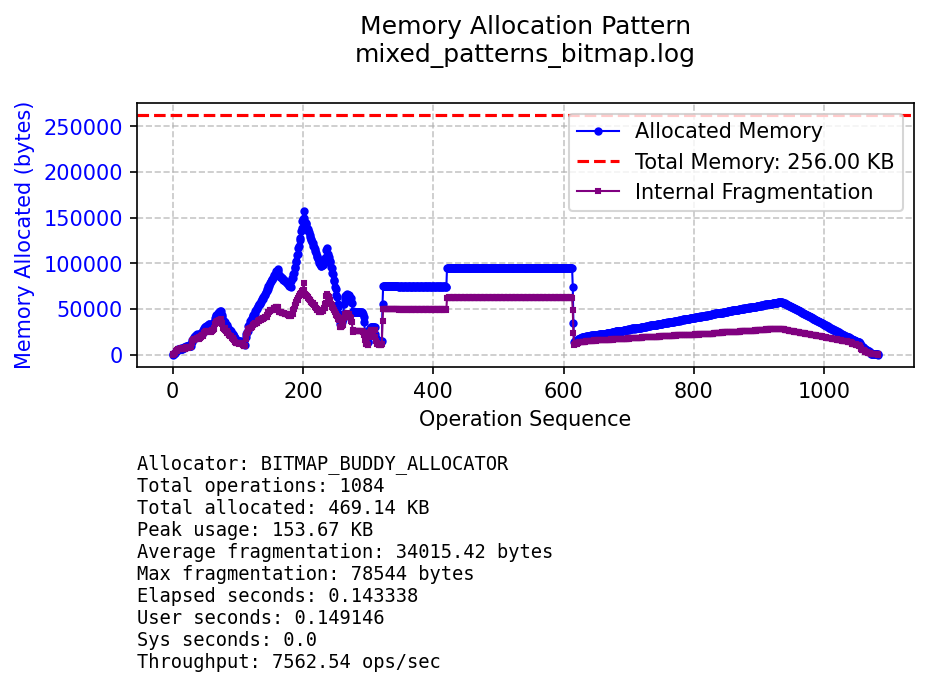
\includegraphics[width=0.9\textwidth]{graphs/mixed_patterns_bitmap.png}
  \caption{Comportamento del BitmapBuddyAllocator su un benchmark contenente in ordine, \textit{peaks, plateaus} e \textit{ramps}.}
  \label{fig:mixed_patterns_bitmap}
\end{figure}




\subsection{Allocazioni sfavorevoli: frammentazione interna}

Come abbiamo menzionato precedentemente nella nostra analisi dell'implementazione degli allocatori che implementano un \textit{buddy system}, la possibilità di frammentazione interna molto elevata al punto da essere debilitante non è da trascurarsi. Adoperando lo strumento da noi creato per simulare un caso estremo, possiamo facilmente osservare dai grafici come determinate combinazioni di parametri di inizializzazione e richieste mal formulate possano rendere l'allocatore molto inefficace nel gestire la memoria a sua disposizione. Le linee rosse sul grafico rappresentano richieste che non è stato possibile soddisfare per via di frammentazione interna o esterna.
\begin{figure}[H]
  \centering
  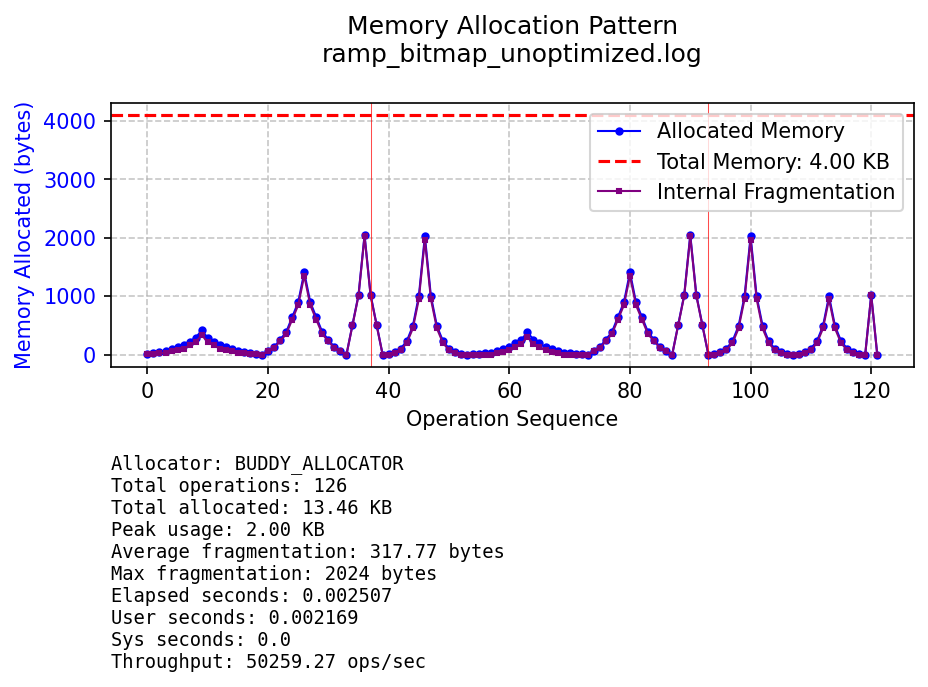
\includegraphics[width=0.9\textwidth]{graphs/ramp_bitmap_unoptimized.png}
  \caption{Sequenza di istruzioni che causano nel BuddyAllocator grande frammentazione interna. Notiamo che la quantità di memoria inutilizzabile è pari a quella allocata.}
  \label{fig:ramp_bitmap_unoptimized}
\end{figure}

Chiaramente, il caso riportato sopra risulta essere manipolato per esasperare il nostro punto. Non vi è alcun dubbio che sarebbe ben difficile incontrare in natura un pattern così sfortunato: tuttavia, bastano una serie di allocazioni mal concepite per rendere, soprattutto in corrispondenza di picchi di utilizzo, una cospicua parte della memoria inutilizzabile e pertanto riteniamo sia importante che il programmatore avveduto faccia uso di strumenti simili per comprendere il comportamento del proprio allocatore e, se necessario, apportare cambiamenti che lo rendano più adatto al proprio caso d'uso. Di seguito riportiamo altri due esempi di pattern in cui tuttavia è stata presa cura di minimizzare la frammentazione diminuendo le taglie degli oggetti allocati oppure, più semplicemente, aumentando di poco la dimensione dell'area di memoria che l'allocatore amministra.

\begin{figure}[H]
  \centering
  \begin{minipage}{0.5\textwidth}
    \centering
    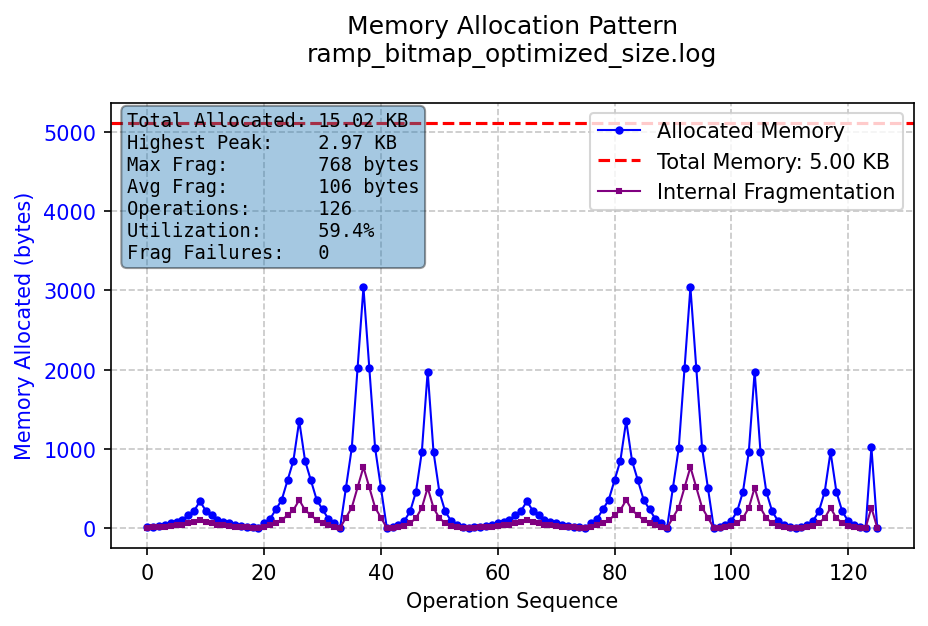
\includegraphics[width=0.95\textwidth]{graphs/ramp_bitmap_optimized_size.png}
    \caption{Con richieste di dimensione leggermente minore, la frammentazione diventa irrilevante.}
    \label{fig:ramp_bitmap_optimized_size}
  \end{minipage}\hfill
  \begin{minipage}{0.5\textwidth}
    \centering
    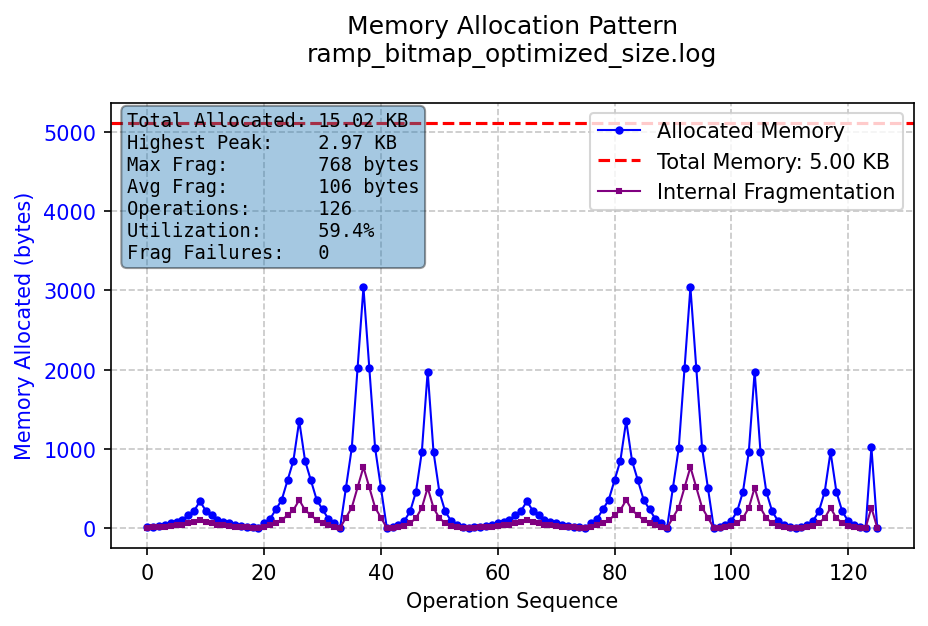
\includegraphics[width=0.95\textwidth]{graphs/ramp_bitmap_optimized_size.png}
    \caption{Allocando relativamente poca memoria in più, la frammentazione diminuisce sostanzialmente.}
    \label{fig:ramp_bitmap_optimized_size}
  \end{minipage}
\end{figure}


\subsection{\textit{LinkedList} vs. \textit{Bitmap}}

Sebbene esse siano quasi uguali in termini di frammentazione interna ed esterna (la politica di allocazione è difatti la medesima), la caratteristica che distigue il \texttt{BuddyAllocator} e il \texttt{BitmapBuddyAllocator} è la struttura dati adoperata per mantenere i riferimenti ai blocchi liberi, in quanto l'implementazione del primo adopera liste concatenate per rappresentare ogni livello. Questa scelta è stata fatta in quanto in ogni momento in ogni lista può essere presente un numero di elementi altamente variabile: la natura delle \textit{LinkedList} le rende quindi particolarmente adatte a svolgere questo ruolo. Ciononostante, nella prima iterazione questo allocatore è andato incontro a una problematica, di cui svolgiamo un'analisi nella sezione successiva.

Utilizzando lo strumento \texttt{cachegrind} e gli altri \textit{tool} compresi in \textit{valgrind}, abbiamo potuto svolgere un analisi più approfondita del comportamento del nostro programma, in particolare rilevando le differenze tra le due implementazioni del \textit{buddy system}. Il comportamento della cache dipende dalle caratteristiche del calcolatore. I test eseguiti di seguito sono stati svolti su un sistema avente le seguenti caratteristiche:
\begin{lstlisting}[language={}]
desc: I1 cache:   32768 B, 64 B, 8-way associative
desc: D1 cache:   32768 B, 64 B, 8-way associative
desc: LL cache:   6291456 B, 64 B, 12-way associative
\end{lstlisting}


\subsubsection*{Prevenzione dei \textit{Double free}}
Un'analisi preliminare delle prestazioni del \texttt{BuddyAllocator} mostra che risulta significativamente più lento rispetto all'alternativa basata su bitmap. Questo dato conferma le aspettative teoriche di una maggiore complessità, ma l'entità della differenza osservata è superiore a quanto previsto e suggerisce la presenza di ulteriori fattori che penalizzano l'efficienza dell'implementazione.

\begin{lstlisting}
i,buddy
p,16276,10
I refs:        13,289,525
I1  misses:         2,910
LLi misses:         2,459
I1  miss rate:       0.02%
LLi miss rate:       0.02%

D refs:         8,944,880  (7,197,682 rd   + 1,747,198 wr)
D1  misses:     1,229,603  (1,217,474 rd   +    12,129 wr)
LLd misses:         6,545  (    1,608 rd   +     4,937 wr)
D1  miss rate:       13.7% (     16.9%     +       0.7%  )
LLd miss rate:        0.1% (      0.0%     +       0.3%  )

LL refs:        1,232,513  (1,220,384 rd   +    12,129 wr)
LL misses:          9,004  (    4,067 rd   +     4,937 wr)
LL miss rate:         0.0% (      0.0%     +       0.3%  )
\end{lstlisting}
\begin{itemize}
  \item \textbf{I refs}: Fetch istruzioni; \textbf{I1/LLi misses}: Mancati accessi cache istruzioni (primo/ultimo livello); \textbf{I1/LLi miss rate}: Percentuale miss cache istruzioni.
  \item \textbf{D refs}: Accessi dati (letture/scritture); \textbf{D1/LLd misses}: Mancati accessi cache dati (primo/ultimo livello, letture/scritture); \textbf{D1/LLd miss rate}: Percentuale miss cache dati.
  \item \textbf{LL refs}: Accessi totali cache ultimo livello; \textbf{LL misses}: Mancati accessi totali; \textbf{LL miss rate}: Percentuale miss cache ultimo livello.
\end{itemize}

Come vediamo facilmente, il programma così formulato ha un altissimo numero di istruzioni che accedono alla memoria, e da un'analisi più approfondita scopriamo che ciò avviene per la maggior parte proprio all'interno della funzione \texttt{list\_find}. Questa funzione è chiamata unicamente all'interno dello \texttt{SlabAllocator}, in particolare come parte delle verifiche di correttezza del programma. 

\begin{table}[H]
\centering
\begin{tabularx}{\textwidth}{|X|c|c|c|}
\hline
\textbf{Funzione} & \textbf{Ir (\%)} & \textbf{Dr (\%)} & \textbf{Dw (\%)} \\
\hline
\texttt{list\_find} & 9,633,626 (72.49\%) & 6,018,037 (83.61\%) & 1,205,430 (68.99\%) \\
\hline
\end{tabularx}
\caption{Profilazione della funzione \texttt{list\_find} in \texttt{double\_linked\_list.c}: Ir = \textit{Istruction, read}, Dr = \textit{Data, read}, Dw = \textit{Data, write}.}
\end{table}

All'interno del \texttt{BuddyAllocator} sono presenti due \texttt{SlabAllocator} per uso interno. Uno di essi in particolare, \texttt{node\_allocator}, si occupa di gestire la memoria necessaria per mantenere i \texttt{BuddyNode}: essi contengono le informazioni sui \textit{buddies} e sono quindi indispensabili. Quando la memoria viene rilasciata nel \texttt{BuddyAllocator}, se due \textit{buddies} sono liberi e pertanto riunificati, i \texttt{BuddyNodes} contenenti le informazioni su di essi vengono a loro volta riconsegnati alla \textit{free list} dello \texttt{SlabAllocator}. Quando esso riprende possesso di uno \textit{slab}, si assicura che esso non sia stato precedentemente rilasciato (evitando l'errore noto come \textit{double free}). La modalità attraverso cui compie questa verifica è la scansione della lista contenente tutti gli slab liberi, ma, poiché  adoperando il \textit{tool} questa soluzione è stata riconosciuta come molto costosa, in quanto il costo chiaramente è lineare al numero degli stessi. Il numero di istruzioni che accedono alla memoria diventa quindi altissimo: l'efficienza ne risente a causa dell'elevato numero di \textit{data cache miss}.

\begin{lstlisting}
  // Check if node is already in free list using list_find
  if (list_find(slab->free_list, &slab_node->node)) {
      #ifdef DEBUG
      printf(RED "ERROR: Failed to free: slab node already in free list!\n" RESET);
      #endif
      return NULL;
  }
\end{lstlisting}

Per evitare la scansione lineare, la soluzione applicata è l'utilizzo di una flag, \texttt{bool in\_free\_list}, che ci permette di verificare più rapidamente se il blocco sia stato già liberato e quindi aggiunto alla \texttt{free list}. Questo \textit{check} tuttavia è molto meno sicuro, e se il dato venisse corrotto permetterebbe il \textit{double free} di uno slab, che potrebbe dunque essere restituito due volte come risultato di una richiesta di memoria. 



\subsubsection{Bitmap e cache}

\begin{lstlisting}[language={}]
i,bitmap
p,16276,10

I refs:        14,221,610
I1  misses:         2,790
LLi misses:         2,460
I1  miss rate:       0.02%
LLi miss rate:       0.02%

D refs:         7,089,558  (4,813,930 rd   + 2,275,628 wr)
D1  misses:         4,567  (    2,269 rd   +     2,298 wr)
LLd misses:         3,405  (    1,616 rd   +     1,789 wr)
D1  miss rate:        0.1% (      0.0%     +       0.1%  )
LLd miss rate:        0.0% (      0.0%     +       0.1%  )

LL refs:            7,357  (    5,059 rd   +     2,298 wr)
LL misses:          5,865  (    4,076 rd   +     1,789 wr)
LL miss rate:         0.0% (      0.0%     +       0.1%  )
\end{lstlisting}


\begin{lstlisting}[language={}]
i,buddy
p,16276,10

I refs:        3,652,823
I1  misses:        2,913
LLi misses:        2,463
I1  miss rate:      0.08%
LLi miss rate:      0.07%

D refs:        1,719,901  (1,178,874 rd   + 541,027 wr)
D1  misses:        7,915  (    2,430 rd   +   5,485 wr)
LLd misses:        6,545  (    1,608 rd   +   4,937 wr)
D1  miss rate:       0.5% (      0.2%     +     1.0%  )
LLd miss rate:       0.4% (      0.1%     +     0.9%  )

LL refs:          10,828  (    5,343 rd   +   5,485 wr)
LL misses:         9,008  (    4,071 rd   +   4,937 wr)
LL miss rate:        0.2% (      0.1%     +     0.9%  )
\end{lstlisting}

\pagebreak

\subsection{Esempi di file \texttt{.alloc}}
\begin{lstlisting}[language={}]
% Tipo di allocatore (Slab)
i,slab         
% Parametri: slab_size=64, num_slabs=16
p,64,16        
% Alloca un blocco nell'indice 0
a,0            
% Alloca un blocco nell'indice 1
a,1            
% Libera il blocco nell'indice 0
f,0      
\end{lstlisting}      
\begin{lstlisting}[language={}]
% Benchmark per allocatore variabile
i,buddy
% memory_size=1024, max_levels=5
p,1024,5       
% Alloca 256 byte nell'indice 0
a,0,256        
% Alloca 128 byte nell'indice 1
a,1,128        
% Libera l'indice 0
f,0            
% Alloca 64 byte nell'indice 2
a,2,64         
\end{lstlisting}
\pagebreak






\chapter{Conclusioni}

Riprendi la dichiarazione d’intenti al capitolo uno e metti le spunte.

\begin{thebibliography}{9}

\bibitem{emeryberger}
  E. Berger, \emph{Malloc Implementations: Historical and Technical Analysis}, GitHub Repository, 2018. \\
  \url{https://github.com/emeryberger/Malloc-Implementations}

\bibitem{bonwick1994}
  J. Bonwick, \emph{The Slab Allocator: An Object-Caching Kernel Memory Allocator}, 1994.

\bibitem{bryant2015}
  R. Bryant, D. O’Hallaron, \emph{Computer Systems: A Programmer’s Perspective (3rd Edition)}, 2015.

\bibitem{chilimbi2000}
  T. Chilimbi, R. Jones, B. Zorn, \emph{Designing a Trace Format for Heap Allocation Events}, 2000. \\
  \texttt{trishulc@microsoft.com}, \texttt{R.E.Jones@ukc.ac.uk}, \texttt{zorn@microsoft.com}

\bibitem{cvut-dynamic-mem}
  \emph{Dynamic Memory Allocation}, Czech Technical University in Prague (CVUT), \\
  \url{https://cw.fel.cvut.cz/old/_media/courses/a4m33pal/04_dynamic_memory_v6.pdf}

\bibitem{anu-malloc}
  \emph{COMP2310: Lab 5 - malloc}, Australian National University, \\
  \url{https://comp.anu.edu.au/courses/comp2310/labs/05-malloc/}

\bibitem{cornell-malloc}
  \emph{CS3410 Project 6: Dynamic Memory Allocation}, Cornell University, 2018. \\
  \url{https://www.cs.cornell.edu/courses/cs3410/2018fa/projects/p6/}

\bibitem{dlmalloc}
  D. Lea, \emph{A Memory Allocator (dlmalloc)}, 1987.

\bibitem{kernighan1988}
  B. Kernighan, D. Ritchie, \emph{The C Programming Language (2nd Edition)}, 1988.

\bibitem{knowlton1965}
  K. C. Knowlton, \emph{A Fast Storage Allocator}, Communications of the ACM, Vol. 8, No. 10, pp. 623–625, 1965.

\bibitem{knuth1997}
  D. Knuth, \emph{The Art of Computer Programming, Volume 1: Fundamental Algorithms (3rd Edition)}, 1997.

\bibitem{mtrebi}
  M. Trebi, \emph{Memory Allocators: Implementations and Comparisons}, GitHub Repository, 2020. \\
  \url{https://github.com/mtrebi/memory-allocators}

\bibitem{epita-malloc}
  \emph{Malloc Tutorial}, École Pour l'Informatique et les Techniques Avancées (EPITA), \\
  \url{https://wiki-prog.infoprepa.epita.fr/images/0/04/Malloc_tutorial.pdf}

\bibitem{puaut2002}
  I. Puaut, \emph{Real-Time Performance of Dynamic Memory Allocation Algorithms}, 2002.

\bibitem{schreiner1994}
  A. Schreiner, \emph{Object-Oriented Programming with ANSI-C}, 1994.

\bibitem{soshnikov-allocator}
  D. Soshnikov, \emph{Writing a Memory Allocator}, 2019. \\
  \url{https://dmitrysoshnikov.com/compilers/writing-a-memory-allocator/}

\bibitem{wilson1995}
  P. Wilson, M. Johnstone, M. Neely, D. Bryant, \emph{Dynamic Storage Allocation: A Survey and Critical Review}, 1995.

\bibitem{wilson1998}
  P. Wilson, M. Johnstone, \emph{The Memory Fragmentation Problem: Solved?}, 1998.

\end{thebibliography}

\backmatter

\begin{acknowledgments}
  ACK HERE 
\end{acknowledgments}

\end{document}